\documentclass[preprint]{article}

%% Define the \sys command for the system name
\newcommand{\sys}{SchedCP\xspace}
%% Define the \agent command for the sched-agent name
\newcommand{\agent}{sched-agent\xspace}


\usepackage{neurips_2025}
% \usepackage[final]{neurips_2025}


\usepackage{listings}     % For ASCII-art / code blocks
\usepackage{booktabs}     % Nicer tables
\usepackage{array}        % Column types
\usepackage{tabularx}     % Automatic column width
\usepackage{enumitem}     % Compact lists



\usepackage{comment}

\usepackage[utf8]{inputenc}
\usepackage[T1]{fontenc}
\usepackage{textcomp}
\usepackage[english]{babel} 
\usepackage{url}
\usepackage{graphicx}


\usepackage{hyperref}       % hyperlinks
\usepackage{amsfonts}       % blackboard math symbols
\usepackage{nicefrac}       % compact symbols for 1/2, etc.
\usepackage{microtype}      % microtypography
\usepackage{xcolor}         % colors




\title{Towards Agentic OS: An LLM Agent Framework for Linux Schedulers}



\author{%
  Yusheng Zheng$^{1}$ \quad
  Yanpeng Hu$^{2}$ \quad
  Andi Quinn$^{1}$ \\
  $^{1}$UC Santa Cruz, CA, USA \quad
  $^{2}$ShanghaiTech University, Shanghai, China \\
  \texttt{\{yzhen165, aquinn1\}@ucsc.edu, huyp@shanghaitech.edu.cn}
}
\sloppy
\begin{document}


\maketitle


\begin{abstract}
Operating system schedulers suffer from a fundamental semantic gap, where kernel policies fail to understand application-specific needs, leading to suboptimal performance. We introduce \sys, the first framework that enables fully autonomous Large Language Model (LLM) agents to safely and efficiently optimize Linux schedulers without human involvement. Our core insight is that the challenge is not merely to \emph{apply} a better LLM, but to architect a decoupled control plane that separates the AI's role of semantic reasoning ("what to optimize") from the system's role of execution ("how to observe and act"). Implemented as Model Context Protocol(MCP) server, \sys provides a stable interface with three key services: a Workload Analysis Engine, an evolving Scheduler Policy Repository, and an Execution Verifier that validates all AI-generated code and configure before deployment with static and dynamic analysis. 

We demonstrate this architecture's power with \agent, a multi-agent system that autonomously analyzes workloads, synthesizes custom eBPF scheduling policies, and deploys them via the sched\_ext infrastructure. Our evaluation shows that SchedCP achieves up to an 1.79x performance improvement, and a 13x cost reduction compared to naive agentic approaches, all while maintaining high success rate. By bridging the semantic gap, SchedCP democratizes expert-level system optimization and represents a step towards creating truly self-optimizing, application-aware operating systems. The code will be open-sourced.
\end{abstract}



\maketitle
\section{Introduction}
\label{sec:intro}

Operating system schedulers face a fundamental challenge: kernel policies cannot understand what applications need. This semantic gap leads to suboptimal performance across modern computing infrastructure. In cloud platforms, system administrators who manage schedulers are not the developers who understand application behavior. On personal devices, regular users lack the expertise to optimize their systems for gaming or creative workloads. Meanwhile, workloads themselves exhibit increasingly dynamic patterns that defy manual optimization.

Prior attempts to automate scheduler optimization, such as those using reinforcement learning~\cite{mao2019decima, qiu2020firm}, have shown promise but remain fundamentally limited. By mapping numerical state to predefined actions, they cannot grasp the semantic intent of a workload and miss optimization opportunities that require deeper reasoning. The advent of Large Language Models (LLMs) Agents, which can automatically reason and use tools for software development, presents an opportunity to bridge this semantic gap, yet a naive approach is impractical. As our motivating experiments reveal, using a powerful agent to generate a basic scheduler from scratch was slow, expensive (\textasciitilde\$6), and resulted in code that often degraded system performance. This highlights a critical gap: existing methods lack semantic understanding, while powerful new models lack the necessary scaffolding for safe, efficient, and reliable systems integration.

To bridge this gap, we introduce a novel, decoupled architecture consisting of two complementary components that leverages AI's unique strengths (semantic reasoning and generative synthesis) while mitigating its weaknesses of cost and unreliability. The first component is \sys, a control plane framework that acts as a safe, stable interface between AI and the kernel. \sys\ provides the essential tools any agent needs to optimize schedulers, including profilers and tracers for observation, and static and dynamic analysis for validation and safe deployment. The second component is \agent, our implementation of an autonomous reinforcement learning policy engine that leverages a multi-agent LLM system. \agent\ uses the capabilities provided by \sys\ to reason about workloads, synthesize policies, and adapts its strategy based on performance feedback. By reducing optimization costs, our approach makes custom scheduler development economically viable even for short-lived workloads like CI/CD pipelines that previously could not justify the engineering investment.

This architectural separation is fundamental to our approach. \sys\ embodies our core systems contribution: a generalizable framework that can work with any future AI agent, while \agent\ demonstrates the power of this approach through semantic workload analysis and intelligent policy generation. The name `\sys` is inspired by "Context Protocol" (like MCP) and the networking concept of a "Control Plane," reflecting its role as a control plane for AI-driven policy orchestration, separate from the data plane where low-level scheduling decisions execute. Deployed on the production-ready sched\_ext infrastructure, our approach executes with zero LLM overhead in the critical path and makes the following contributions:

\begin{itemize}
    \item \textbf{The \sys\ interface}: A framework that exposes kernel scheduling related features via the Model Context Protocol (MCP), featuring three core services (Workload Analysis Engine, Scheduler Policy Repository, and Execution Verifier) that enable any agent to perform deep semantic analysis of workloads, do AI-driven scheduler optimization without compromising system stability, and learns from experience and improve performance over time.
    \item \textbf{\agent\ multi-agent system}: An autonomous reinforcement learning policy engine that decomposes scheduler optimization into four specialized agents (Observation, Planning, Execution, and Learning), demonstrating how LLMs can bridge the semantic gap between application requirements and kernel scheduling policies.
    \item \textbf{Evaluation}: We demonstrate that \agent\ achieves up to 1.79× performance gains on kernel compilation, 2.11× P99 latency improvement and 1.60× throughput gain on schbench, 20\% average latency reduction for batch workloads, and 13× lower cost compared to naive approaches, while maintaining system stability across diverse workloads.
\end{itemize}

Paper organization: Background (§\ref{sec:background}), Motivation (§\ref{sec:motivation}), \sys (§\ref{sec:schedcp_framework}), \agent (§\ref{sec:sched_agents}), Evaluation (§\ref{sec:evaluation}), Related Work (§\ref{sec:related}), Future Work (§\ref{sec:future}), and Conclusion (§\ref{sec:conclusion}).
\section{Background}
\label{sec:background}

This section reviews the two core technologies for our work: extensible kernel scheduling and autonomous LLM agents.

\subsection{eBPF and sched\_ext}

Linux's default Earliest Eligible Virtual Deadline First (EEVDF) scheduler~\cite{eevdf2024}, which replaced CFS in kernel 6.6, is a one-size-fits-all policy that, while ensuring fairness through virtual deadlines, is unoptimized for diverse workloads. To address this, sched\_ext~\cite{schedext2024}, introduced in Linux 6.12, enables the dynamic loading of custom schedulers as eBPF programs, providing hooks for task enqueueing, CPU selection, load balancing, and idle management. This relies on eBPF~\cite{ebpfio}, which evolved from a simple packet filter into a general-purpose, in-kernel virtual machine. Now powering modern observability and security tools~\cite{tracee,cilium} on both Linux and other systems like Windows and userspace~\cite{zheng2025extending, windows-ebpf}, its verifier guarantees safety through static analysis, preventing crashes, invalid memory access, and infinite loops. Previous work also explores using LLM for eBPF code generation\cite{kgent}.

\subsection{LLMs and Autonomous Agents}

The application of large language models (LLMs) like GPT-4~\cite{openai2023gpt4} and Claude~\cite{anthropic2024claude} has evolved from code generation to system maintenance~\cite{de2025llm} and fully autonomous agents. These agents typically use an architecture with an LLM backend, a tool framework, and a control loop, as seen in popular frameworks like LangChain~\cite{langchain}, AutoGen~\cite{autogen} and commercial tools like Cursor Agent~\cite{cursor}, Gemini-CLI~\cite{geminicli}, and Claude Code~\cite{claudecode} for automate software engineering workflows. Further research into multi-agent frameworks like ChatDev~\cite{qian2024chatdev} and MetaGPT for software development~\cite{hong2023metagpt}, repo understanding~\cite{coderesearcher2025}, and simulate social behaviors~\cite{agent4se2024} has shown that role-playing can boost code generation and issue localization~\cite{Lin2025FlowGen,Batole2025LocalizeAgent}. Despite these advances, the tools remain developer aids, not autonomous low-level system optimizers.
\section{Motivation}
\label{sec:motivation}

We motivate our work by examining this semantic gap problem and the practical safety, performance, and cost issues revealed by our experiments.

\subsection{The Semantic Gap Problem}

\textbf{Domain Knowledge Gap between developer and user}: In cloud environments, DevOps engineers configuring Kubernetes lack insight into workload characteristics (latency-sensitive vs. throughput-oriented), resulting in conservative scheduling. Edge and personal devices face worse challenges. Gamers, creative professionals, and office workers lack kernel expertise for optimization. LLMs can bridge this gap by understanding high-level workload patterns from source code and deployment artifacts, and translating them into concrete scheduling policies.

\textbf{Technical Complexity of Scheduler Development}: Linux scheduler development requires mastering kernel programming with lock-free structures, eBPF verification constraints, and CPU/NUMA architectures. This steep learning curve limits innovation to few kernel experts. LLMs with pre-trained domain knowledge enable rapid and automated scheduler development without human expertise.

\textbf{Dynamic Workload Adaptation}: Modern workloads exhibit complex phase behavior: ML training alternates between compute-intensive forward propagation and communication-heavy gradient synchronization; web traffic varies by orders of magnitude daily; build system parallelism changes with dependencies. Manual reconfiguration and optimization cannot keep pace, while AI agents can adapt policies in real-time, operating 24/7 without breaks, much more availability than human experts.

\subsection{Economic Viability of AI-Driven Scheduler Optimization}

Scheduler optimization becomes economically viable when generation costs are lower than CPU time savings. For example, with \$0.45 AI generation LLM API cost and 20\% performance improvement, a 10-hour workload on a \$2/hour instance already breaks even (\$0.45 cost vs \$4 savings). This fundamentally changes scheduler economics: traditionally, high manual engineering costs meant custom schedulers were only justified for large-scale cloud workloads running on hundreds of machines for months, but AI assistance now makes it economical to optimize even short-lived workloads like CI/CD pipelines, batch jobs, or individual builds running for just hours or days on single machines, democratizing performance optimization for previously uneconomical use cases.

\subsection{Motivation Experiment}

We tested Claude Code\cite{claudecode}, the state of the art LLM agent, with "write a FIFO scheduler in eBPF" from an empty folder, with all permissions and bash access. Of three attempts, only one succeeded. The second attempt produced pseudo-code after 6 minutes trying, and the third generated a scheduler tracer instead after 8 minutes development. The successful generation required 33 minutes, 221 LLM API calls, and 15+ iterations, costing \$6 (vs. 5 minutes typically for an expert developer). The generated code, for some workloads, exhibited poor quality with excessive overhead, performing worse than EEVDF. The agent required root access, could crash the system during testing, and lacked fallback mechanisms, which also raises safety concerns.

\subsection{Challenges in Applying LLM Agents to Schedulers}

Our experiments reveal critical challenges for AI-driven scheduler optimization, especially when fully automated: \textbf{Performance}: How do we ensure AI-generated or configured schedulers outperform existing ones rather than degrading performance? \textbf{Safety}: How do we prevent kernel crashes, soft-lockups, stalls, or starvation while maintaining stability? How can we ensure only minimal privilege needed when development and deployment? \textbf{Efficiency}: The 33-minute generation time and the \$6 cost must drop for practical deployment.
\section{The \sys\ Framework Design and Implementation}
\label{sec:schedcp_framework}

\begin{figure}
    \centering
    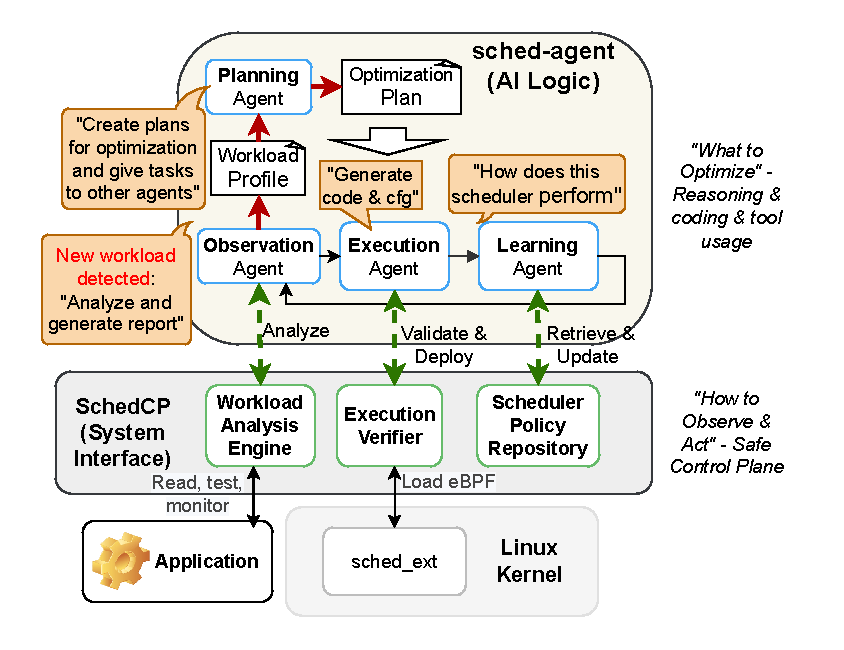
\includegraphics[width=\columnwidth]{sections/img/arch-scheddcp.pdf}
    \caption{
        \textbf{The overall architecture, showing the separation of concerns between \sys\ and \agent } 
        The \textbf{\sys} framework (bottom) acts as a safe system interface, providing tools to analyze workloads, verify code, and manage scheduler policies in the Linux kernel via eBPF.
        The \textbf{\agent} framework (top) contains the AI logic, where specialized agents for Observation, Planning, Execution, and Learning collaborate in a closed loop to autonomously create, deploy, and refine scheduling policies. The red line indicate the initialize process When \sys detects a new workload. The back arrow indicate the optimization loops, where \agent continue refines scheduler policies based on optimization plan and observation results. The Green arrows indicate the tool usage by the AI Agents.
    }
    \label{fig:frameworkarch}
\end{figure}

Our approach to agentic OS optimization is founded on a clean separation between the systems infrastructure and the AI logic, as illustrated in Figure~\ref{fig:frameworkarch}. We introduce \sys, a stable and secure control plane that acts as an 'API for OS optimization.' Our research is motivated by the insight that AI agents are fundamentally context engineering systems; like human experts, they need the right tools to gather information and act without being overwhelmed by prohibitive costs or irrelevant data. Therefore, as system researchers, our goal is not to build better AI agents, but to design superior systems and interfaces for them. \sys embodies this by providing the essential tools and safety guarantees for any agent to interact with the Linux kernel's scheduler, analogous to how an environment in reinforcement learning provides the state, actions, and rewards for an agent to learn. This section details \sys's design principles, core components, and implementation. \sys is implemented in ~4000 lines of Rust and ~6000 lines of python (Include tests).

\subsection{Design Principles}
The design of \sys\ is governed by four key principles that ensure it is safe, efficient, and future-proof.

\textbf{Decoupling and Role Separation}: A system tightly coupled to a specific AI model's capabilities will quickly become obsolete as models evolve. To ensure our framework is future-proof, we believe the system's role must be separated from the AI's. Our principle is to decouple ``what to optimize'' (the AI's domain) from ``how to observe and act'' (the system's domain). We treat the AI agent as a performance engineer using a stable set of tools provided by the system, allowing the framework to remain relevant even as AI capabilities advance.

\textbf{Safety-First Interface Design}: Autonomous agents with kernel access pose inherent risks. System stability is non-negotiable, so we treat AI as potentially non-cautious actors and design defensive interfaces. The framework prevents catastrophic failures by default rather than trusting agents to avoid them.

\textbf{Context and Feedback Balance}: LLM agents face constraints from finite context windows and token costs. Performance degrades when flooded with irrelevant data. We address this through adaptive context provisioning: agents start with minimal summaries and progressively request details as needed, balancing cost against precision.

\textbf{Composable Tool Architecture}: Rigid workflows stifle LLMs' ability to reason and devise novel solutions. Following Unix philosophy, we provide atomic tools and let agents construct complex workflows through their reasoning capabilities, enabling novel solution generation.

\subsection{Core Components and Implementation}
\sys is engineered as a modular control plane, exposing its services to AI agents via the standard Model Context Protocol (MCP)~\cite{anthropic2024mcp}. This design cleanly separates the high-level policy orchestration managed by the agent from the low-level observation and execution handled by the framework, and avoids granting `root' privileges to the agent. The architecture consists of three primary services.

\textbf{1. Workload Analysis Engine.} This service provides agents with tiered access to system performance data. It offers three levels of information: (1) cost-effective API endpoints delivering pre-processed summaries like CPU load and memory usage, (2) secure sandbox access to basic file reading, application building, standard Linux profiling tools (\texttt{perf}, \texttt{strace}) and dynamically attachable eBPF probes for detailed analysis, and (3) a feedback channel that reports post-deployment performance metrics such as percentage change in makespan or latency. The service implements adaptive context provisioning, allowing agents to request progressively detailed information as needed.

\textbf{2. Scheduler Policy Repository.} This service is a vector database storing eBPF scheduler code with rich metadata: natural language descriptions, target workloads, and historical performance metrics. It also includes a set of executable scheduler programs. It provides APIs for semantic search and retrieval, enabling agents to find relevant schedulers or composable code primitives. To support system evolution, it includes endpoints for updating performance metrics and promoting new policies. The repository reduces generation costs by allowing reuse of proven solutions while maintaining a growing library of scheduling strategies.

\textbf{3. Execution Verifier.} This validation pipeline service provides multi-stage verification for all AI-generated code and config, beginning with the kernel's standard eBPF verifier to guarantee fundamental memory safety and termination. However, because the standard verifier is agnostic to scheduling logic, it cannot detect flaws like task starvation or unfairness; therefore, our pipeline adds a crucial second layer of scheduler-specific static analysis checkers using customize PREVAIL verifier\cite{prevail} to check for these Correctness and Logic Bugs. Code that passes both static analysis layers proceeds to dynamic validation, where it is compiled and executed within a secure micro-VM against correctness and performance tests. Upon success, the service issues a signed deployment token for a monitored canary deployment, which includes a circuit breaker to automatically revert to the last known-good scheduler if performance degrades, ensuring all policies are rigorously vetted before production use. It also ensures the \agent don't need root access to deploy eBPF schedulers.

\section{\agent: A Multi-Agent Framework for OS Optimization}
\label{sec:sched_agents}

Building on \sys, we developed \textbf{\agent}, a multi-agent AI framework for scheduler optimization. At its core, \agent\ implements in-context reinforcement learning (ICRL)\cite{incontextrl}, a paradigm where the agent adapts its strategy based on recent performance feedback in the context without costly model retraining. We realized this framework using Claude Code's subagent architecture\cite{anthropic2024subagents}, which provides specialized AI assistants with customized system prompts, tools, and separate context windows\cite{anthropic2024multiagent}. Mirroring the collaboration of expert human teams, this multi-agent structure naturally decomposes the complex optimization process into the distinct stages of the ICRL loop: observation (state), planning/execution (action), and learning (reward analysis).

To automatically trigger optimization, \sys integrates with container orchestrators and runtime like Kubernetes and Docker, enabling it to initiate the \agent's analysis cycle whenever a user deploys a new application. It can also be trigger mannually by user.

\subsection{Agent Roles and Responsibilities}

\subsubsection{Observation \& Analysis Agent - Building a Workload Profile}

The \textbf{Observation Agent} builds a comprehensive ``Workload Profile'' by strategically querying the Workload Analysis Engine. Its reasoning process determines the analysis sequence: starting with high-level summaries, then requesting deeper profiling based on initial findings. For example, after identifying a parallel build process through initial queries, the agent decides to request CPU statistics via \texttt{perf stat} and dependency traces via \texttt{strace}. The agent synthesizes these data points into a description of the workload in natural language, quantified performance characteristics, and explicit optimization goals. It manages the cost-precision tradeoff by requesting only essential information and can register for event notifications in \sys to trigger re-analysis when workload patterns change.

\subsubsection{Planning Agent - Policy Synthesis and Selection}

The \textbf{Planning Agent} transforms the Workload Profile into an optimization strategy. It constructs semantic queries for the Scheduler Policy Repository based on the profile's keywords and performance goals. The agent's decision logic follows a hierarchy: search for exact matches, broaden to similar patterns if needed, then decide among three pathways. For existing production-ready scheduler solutions with strong performance history, it configures parameters. For partial matches, it retrieves code and generates patches. When no suitable base exists, it composes new schedulers from algorithm primitives. The agent evaluates tradeoffs between reuse efficiency and customization needs using historical performance data from the repository.

\subsubsection{Execution Agent - Validated Policy Deployment}

The \textbf{Execution Agent} manages the development, validation and deployment process. It synthesizes code artifacts based on the Planning Agent's strategy, then submits them to the Execution Verifier. The agent interprets validation results and adapts accordingly: when static analysis fails, it refines the code; when dynamic tests fail, it analyzes errors and fixes logic issues. The agent decides whether to proceed, retry, or abandon approaches based on verifier feedback. Upon receiving a deployment token, it initiates canary rollout. If the circuit breaker triggers, the agent captures failure context and determines next steps, either revising the approach or escalating to the Learning Agent.

\subsubsection{Learning Agent - Performance Analysis and Knowledge Update}

The \textbf{Learning Agent} completes the in-context reinforcement learning loop and analyzes deployment outcomes to improve future performance. It retrieves metrics from the Feedback Channel and identifies success patterns and failure modes. For immediate benefit, it informs subsequent optimization cycles within the current session. For long-term improvement, it updates the Scheduler Policy Repository: refining performance metrics, annotating schedulers with deployment contexts, and promoting successful novel policies. The agent documents antipatterns from failures to prevent repetition. This dual approach enables both in-session adaptation and persistent system-wide learning.


\subsection{Example: Kernel Compilation}

To illustrate how these four agents work together, consider a kernel compilation workload. The \textbf{Observation Agent} begins by analyzing the Linux kernel source tree, executing \texttt{make -j} to understand the build process, and running \texttt{perf stat} to profile resource usage. This observation produces a Workload Profile: ``CPU-intensive parallel compilation task with short-lived processes, inter-process dependencies, and a goal to minimize makespan.'' During planning, the \textbf{Planning Agent} queries the Scheduler Policy Repository with keywords like ``throughput'' and ``compilation,'' retrieving \texttt{scx\_rusty} as a starting point. It generates a patch to make the scheduler dependency-aware. In execution, the \textbf{Execution Agent} submits the patched code to the Execution Verifier for validation, receiving a deployment token upon success. Finally, after deployment, the \textbf{Learning Agent} receives feedback that the revision achieved a 45\% reduction in makespan, contributing the improved scheduler back to the Scheduler Policy Repository for future use. This entire workflow demonstrates how \agent\ enables AI agents to autonomously optimize system performance through iterative refinement.
\section{Evaluation}
\label{sec:evaluation}

% \subsection{Research Questions}

We investigate key research questions to validate the effectiveness and efficiency of \sys:

\begin{itemize}
\item \textbf{RQ1}: Can \sys effectively configure existing schedulers?
\item \textbf{RQ2}: Can \sys generate new schedulers for specific workloads?
\item \textbf{RQ3}: What is the cost and efficiency of \sys's scheduler generation?
\item \textbf{RQ4}: How much can \agent continue to improve performance after initial attempt?
% \item \textbf{RQ5}: How effectively can \sys understand workloads?
\end{itemize}

\subsection{Experimental Setup}

We evaluate \sys on two machines, machine 1 is an 86-core, 172 threads Intel Xeon 6787P with 758GB RAM, NVMe SSDs, 10Gbps network, with 2x 256 GB CXL (Compute Express Link) memory device, 3 numa node, running Linux 6.14 with sched\_ext. Machine 2 is an 8-core, 8 threads Intel Core Ultra 7 258V with 30GB RAM, NVMe SSDs, 1 NUMA node, running Linux 6.13 with sched\_ext. We test Claude Code (Opus 4) as AI agents to validate framework generality. For each case, we test 3 times and get the average results. In all the experiments, the Agent successfully creates working custom scheduler configurations or eBPF programs.

\subsection{Performance Impact of AI-Driven Optimization}

% For schbench, the LLM achieves 50\% lower p99 latency and 30\% higher throughput by selecting scx\_layered. 

We evaluate the \sys and \agent's ability of effectively configure existing scheduler and learn after first attempt. The Linux kernel build benchmark compile the kernel 6.14 with tinyconfig and ``make -j 172'' on machine 1. Figure~\ref{fig:performance-comparison} shows performance improvements across three stages: baseline EEVDF, LLM-configured schedulers, and Iteration-improved configurations. We also compare with basic RL algorithms that have been proposed for scheduler optimization~\cite{corbet2025ml}, which only tunes scheduler parameter. The workload shows 1.63x speedup from 13.57s to 8.31s using scx\_rusty as the first attemp. After 3 iteration of observe-optimization process, the \agent selects the scx\_layered scheduler and adds 16\% additional gain beyond LLM configuration, with total improvements of 1.79x over baseline EEVDF. In contrast, basic RL approaches show no improvement in our tests, likely because they require hardware-specific retraining, which is costly and time-consuming.

\begin{figure}[h]
\centering
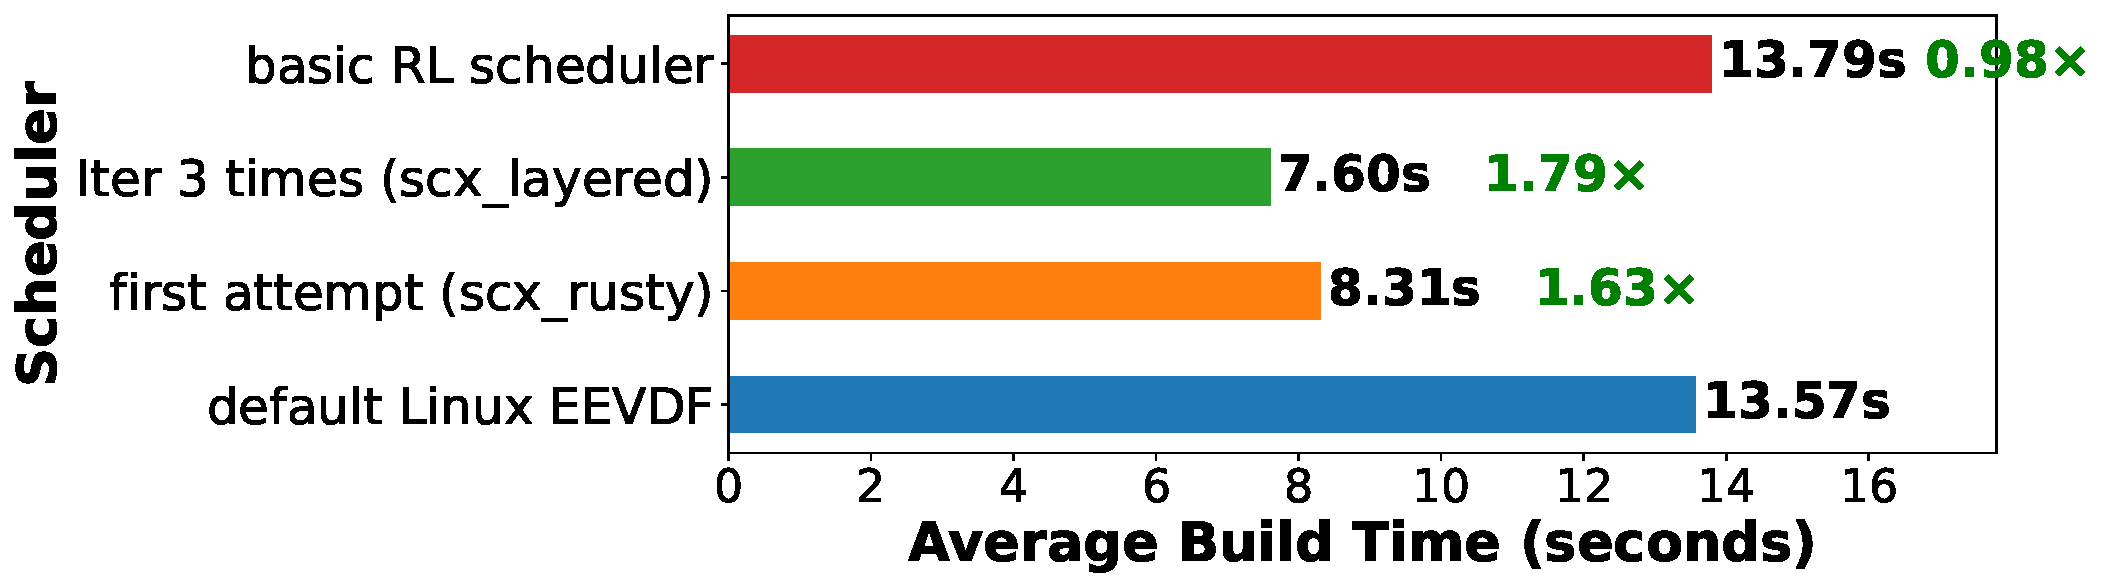
\includegraphics[width=0.9\columnwidth]{sections/Linux_build_benchmark_results.pdf}
\caption{Performance comparison of scheduler configurations in Linux build benchmark.}
\label{fig:performance-comparison}
\end{figure}

We further evaluate \sys on machine 2 using schbench~\cite{schbench2016}, a scheduler benchmark measuring wakeup latency and throughput. Figure~\ref{fig:schbench-comparison} compares three configurations: default EEVDF, initial selection (scx\_bpfland), and iterative optimization (scx\_rusty after 3 iterations). While AI configured scheduler initially underperformed with 13\% worse P99 latency (46.1ms vs 40.3ms) and 19\% lower throughput (741 vs 910 req/s), AI iterative refinement identified scx\_rusty as superior. After three iterations, scx\_rusty achieved 2.11× better P99 latency (19.1ms) and 1.60× higher throughput (1452 req/s) versus EEVDF, demonstrating our agent's effective learning from performance feedback.

\begin{figure}[h]
\centering
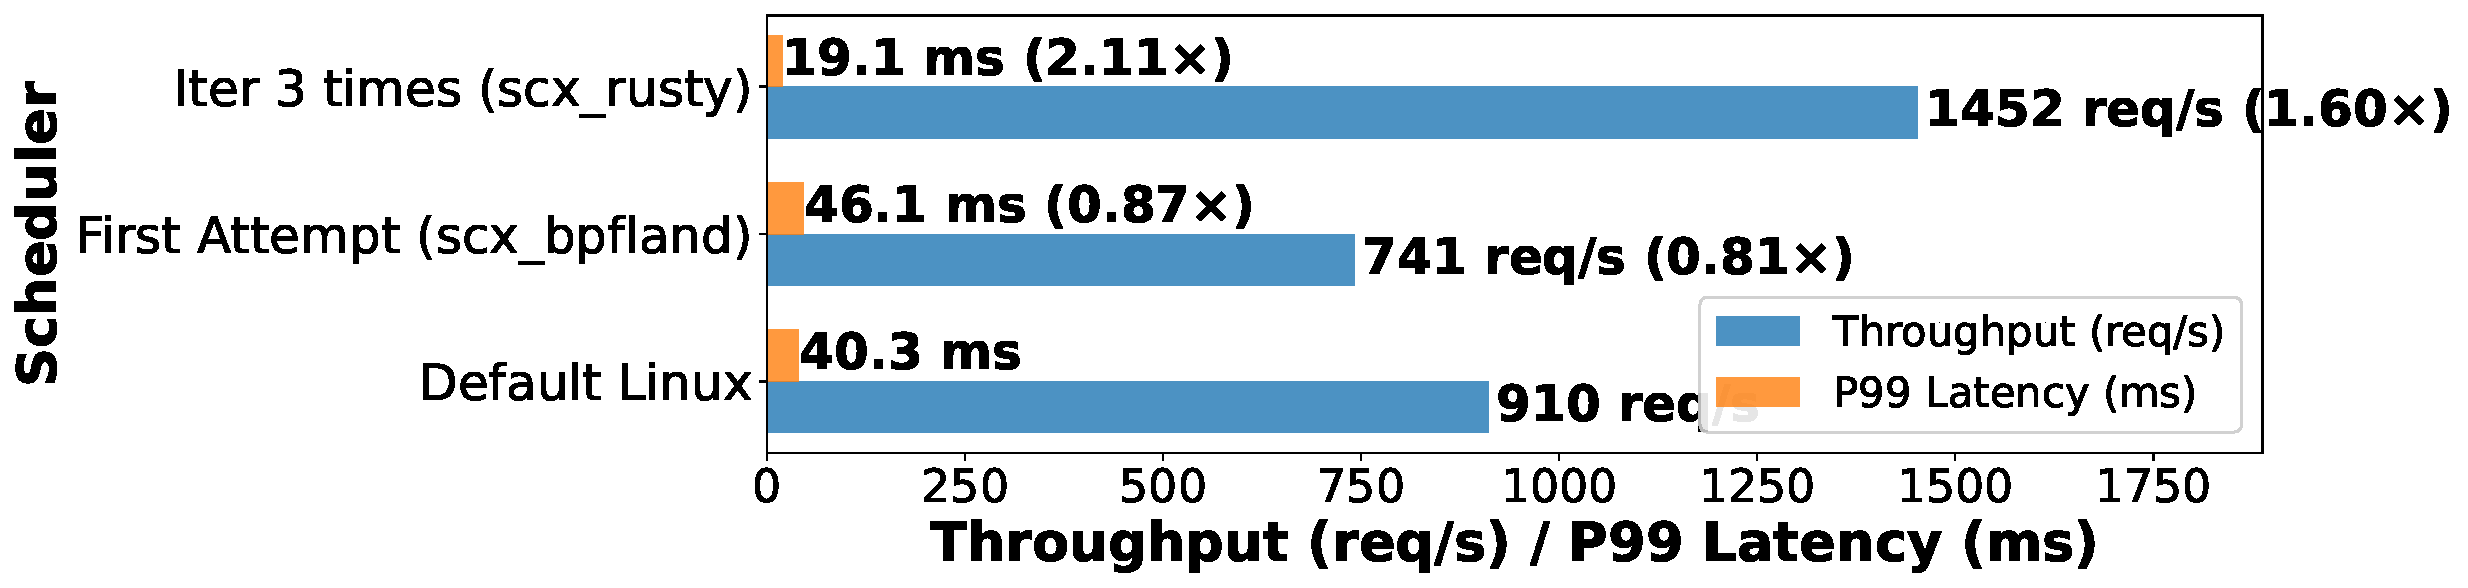
\includegraphics[width=0.9\columnwidth]{sections/schbench_performance_comparison.pdf}
\caption{Schbench performance comparison showing P99 latency and throughput improvements through iterative scheduler optimization.}
\label{fig:schbench-comparison}
\end{figure}

\subsection{Scheduler Synthesis for Batch Workloads}

Figure~\ref{fig:batch-performance} evaluates the \sys  and \agent  ability of generating new and better scheduler from scratch on 8 diverse batch workloads (e.g. file compression, video transcoding, software testing, and data analytics tasks) running on machine 2. To simulate a long-tail distribution, each workload comprised 40 parallel tasks: 39 short and one significantly longer, each as a python script or C/C++ program. The agent consistently identified this pattern, implemented a Longest Job First (LJF) scheduling policy, and achieved an average 20\% reduction in end-to-end processing time. The cost for this analysis averaged \$0.15 per workload, based on Claude Opus 4 pricing from August 2025. We note that the powerful Claude Opus agent successfully classified all 8 workloads, whereas the smaller Claude Sonnet model could not. In addition to performance gains, our framework's optimizations reduced generation costs per iteration: time fell from 33 to 2.5 minutes (a 13x reduction), and the monetary cost dropped from \$6 to \$0.5.

\begin{figure}[h]
\centering
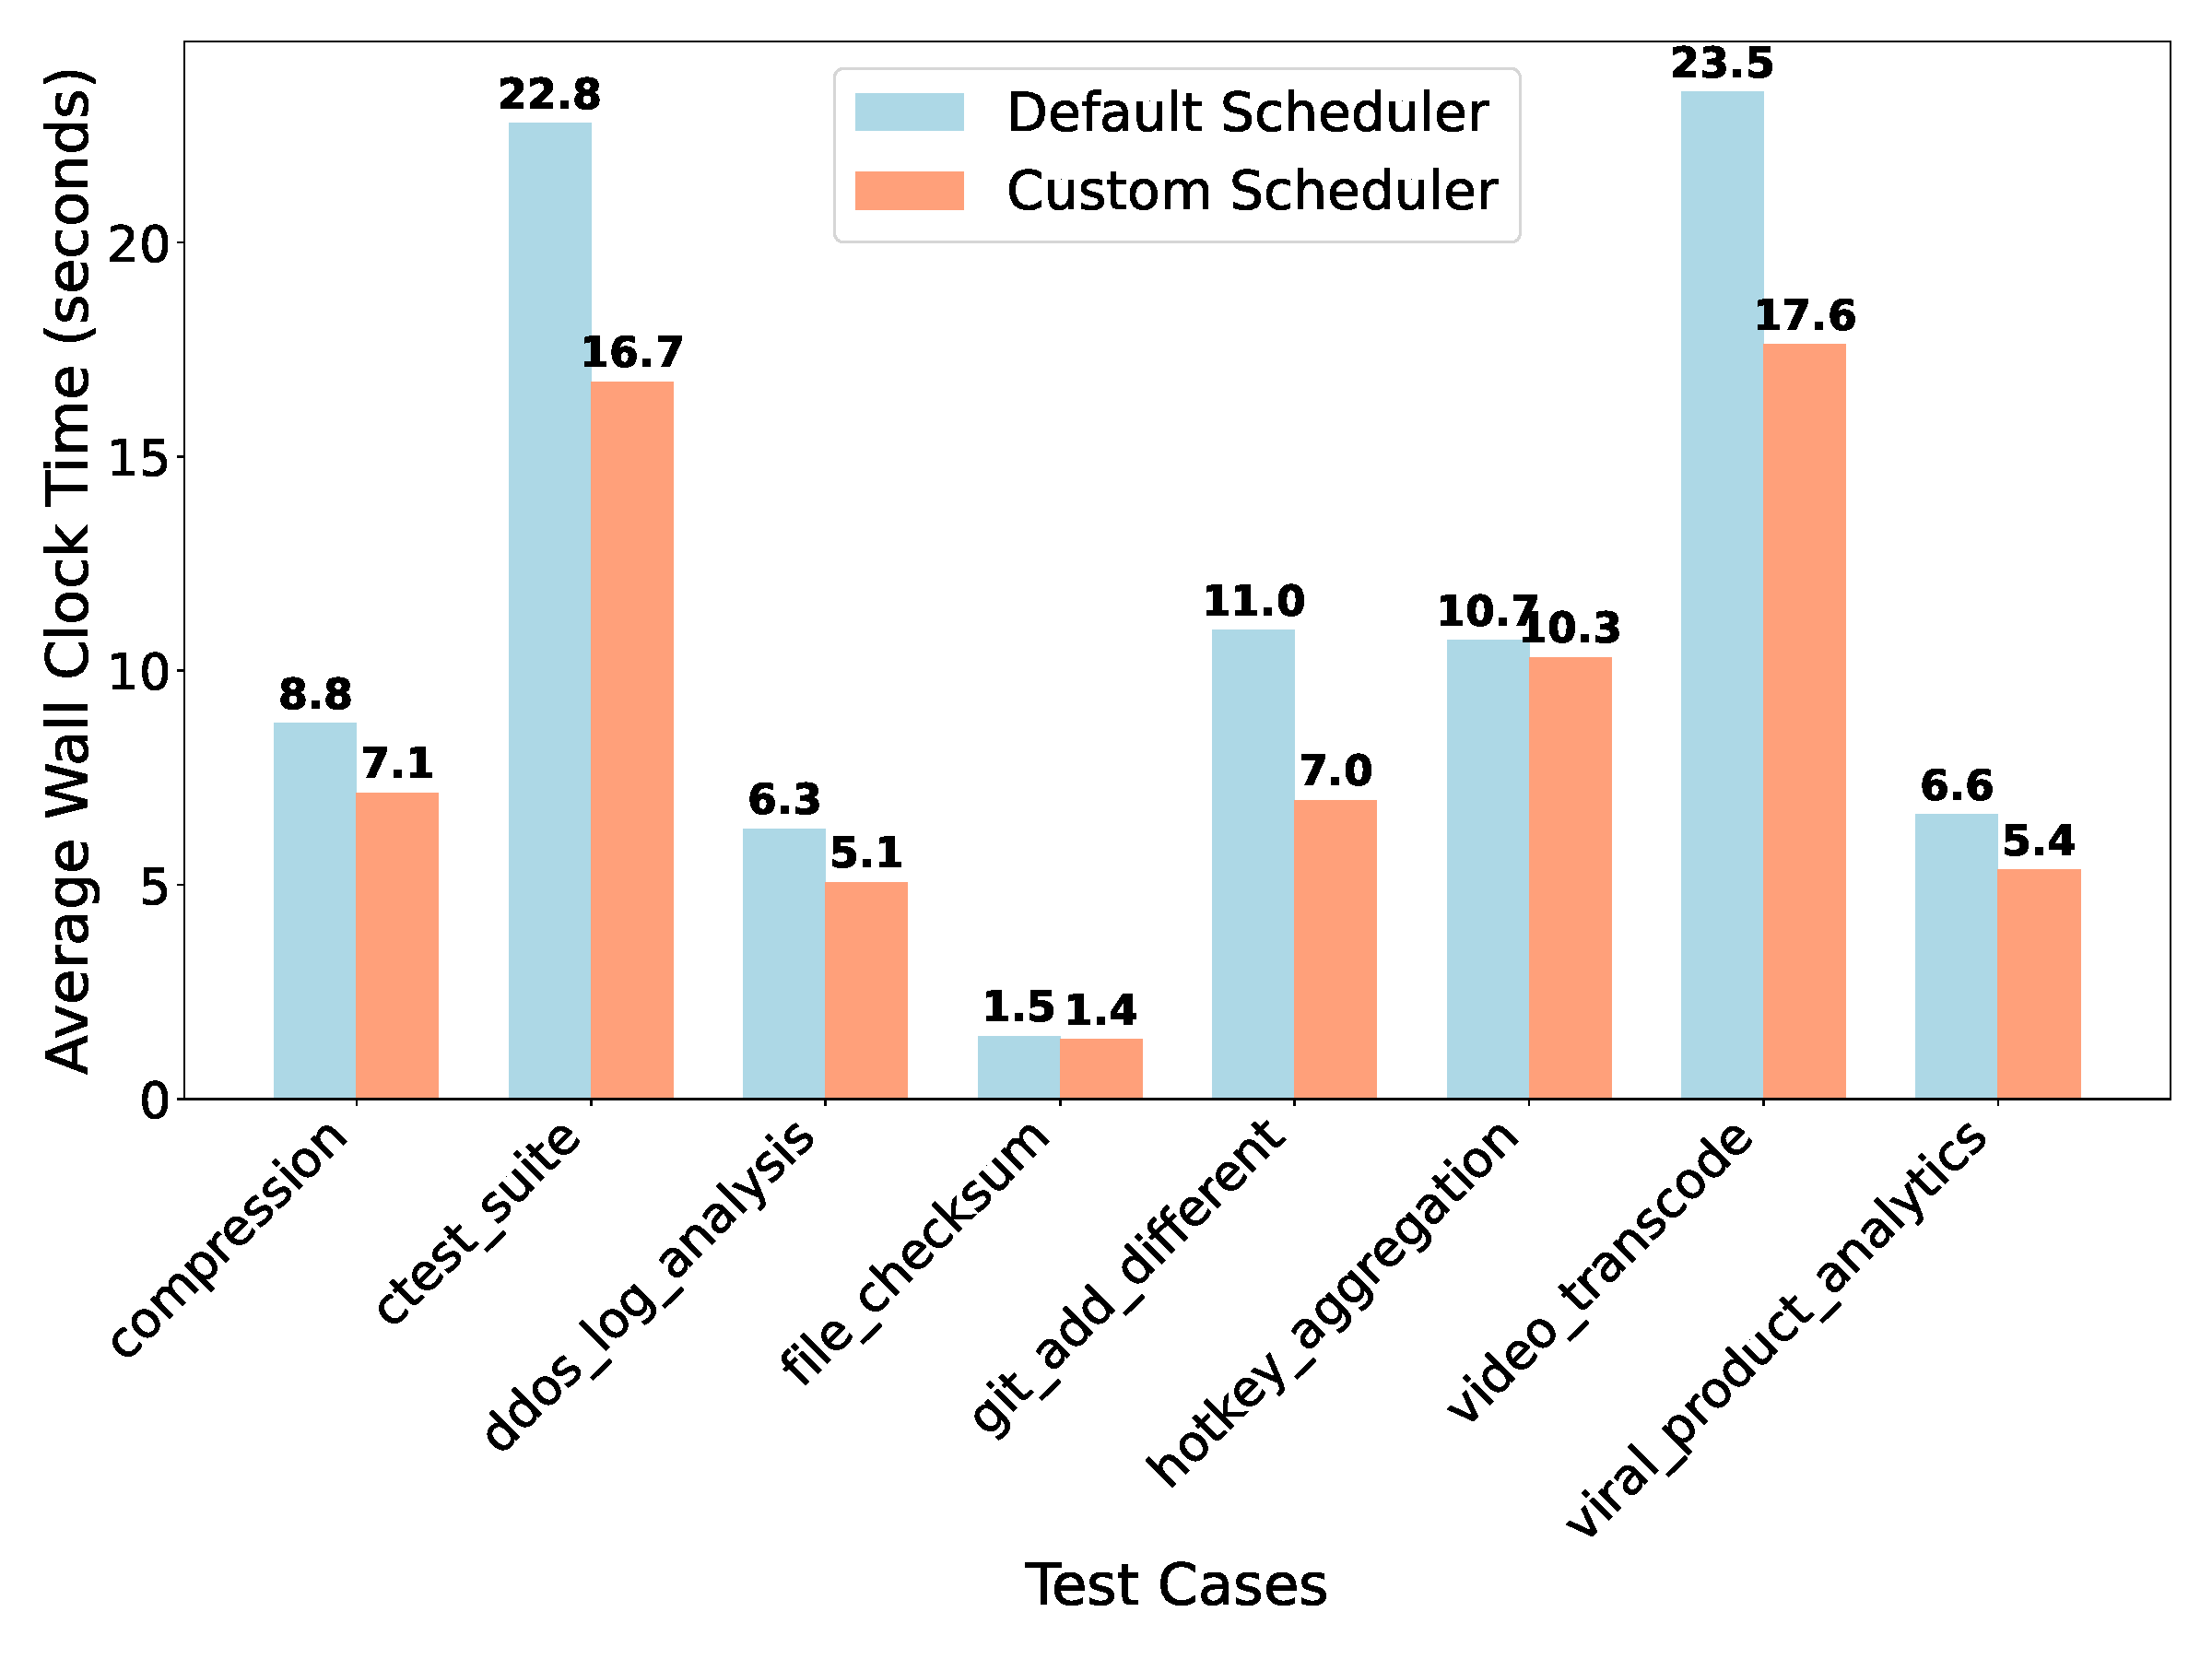
\includegraphics[width=0.9\columnwidth]{sections/scheduler_performance_comparison.pdf}
\caption{AI-generated scheduler performance on batch workloads.}
\label{fig:batch-performance}
\end{figure}
\section{Related Work}
\label{sec:related}

Machine learning has a history of optimizing systems, including learned indexes~\cite{kraska2018learned}, database tuning~\cite{marcus2019neo,vanaken2017ottertune}, and RL-based job schedulers~\cite{mao2019decima,qiu2020firm,zhang2024mrsch} supported by platforms like Park~\cite{mao2019park}. However, these methods require extensive training, lack the semantic understanding to transfer knowledge across diverse workloads, or need human specify high level optimization goals. While recent work has applied LLMs to system diagnostics~\cite{wang2024llmsys} and  code generation~\cite{wei2024mapper,10.1145/3672197.3673434}, our work is the first to use an autonomous agent to design, configure and generate kernel schedulers, and apply them for end-to-end system optimization without human involvement. By leveraging LLM Agent reasoning, tool usage with sched\_ext and eBPF, our framework uniquely bridges the semantic gap between application needs and system policy.
\section{Future Work}
\label{sec:future}

While \sys demonstrates the viability of AI-driven scheduler optimization, extending our framework beyond schedulers to cache policies, DVFS, network configuration, and sysctl parameters presents immediate opportunities for a unified OS optimization framework. Cross-component optimization, where CPU, memory, I/O, and power decisions inform each other, could unlock significant performance gains through new abstractions for expressing inter-component dependencies. This work opens new possibilities for adaptive, application-aware operating systems that can automatically optimize themselves for changing workloads, making expert-level performance accessible to all users.
\section{Conclusion}
\label{sec:conclusion}

We introduce \sys, the first framework for autonomous LLM agents to safely optimize Linux schedulers. Its decoupled control plane separates AI reasoning from safe system execution, bridging the gap between application needs and kernel policy. Our agent, \agent, achieved up to a 1.79× speedup and a 13x cost reduction over naive approaches by autonomously generating and deploying custom eBPF scheduling policies while ensuring stability. SchedCP offers a stable interface for AI-driven optimization, marking a foundational step towards truly application-aware, self-optimizing operating systems.


\bibliographystyle{plain}
\bibliography{sample-base}






\end{document}